\documentclass[11pt]{book}
\usepackage{graphicx}
\usepackage[dvipsnames]{color}
\usepackage[hidelinks]{hyperref}
\usepackage[square,numbers]{natbib}
%pPara poder modificar los margenes
\usepackage{vmargin}
%Para usar el español
\usepackage[spanish]{babel}
\usepackage[utf8]{inputenc}
\usepackage{lscape}
\usepackage{hyperref}
\bibliographystyle{plain}
\begin{document}
%Portada
\setpapersize{A4}
\begin{titlepage}
	\centering
	{
\includegraphics[width=0.8\textwidth]{logo}\par}
	\vspace{1cm}
	{\Large Facultad de Informática \par}
	\vspace{3cm}
	{\scshape\Huge Aplicación web de soporte al Aprendizaje-Servicio \par}
	\vspace{5cm}
	{\textbf\Large Autores \par}
	{\Large Daniela-Nicoleta Boldureanu (Grado en Ingeniería del Software)\par}
	{\Large Victoria Gnatiuk Romaniuk (Grado en Ingeniería Informática)\par}
	{\Large Jesús Sánchez Granado (Grado en Ingeniería Informática)\par}
	\vspace{1cm}
	{\textbf\Large Directores \par}
	{\Large Simon Pickin \par}
	{\Large Manuel Montenegro Montes \par}
	
\end{titlepage}

%Indice

\tableofcontents
\newpage
\listoffigures

\chapter{Introducción}
El objetivo de este \textit{Trabajo de Fin de Grado} (TFG) es retomar la idea de creación de una comunidad web de proyectos ApS (\emph{Aprendizaje-Servicio}) empezada a nuestro saber, en el año 2004 por Emmanuel Parmentier en su (\emph{Proyecto Fin de Carrera}) PFC. Otros trabajos despues siguieron esta trayectoria y el último de ellos fue el TFG de David Jiménez del Rey, este es el proyecto que nosotros continuamos en nuestro TFG. Estos proyecto precedentes se detalla más adelante en el capítulo \ref{cap:cont-motidvacion}. El proyecto objetivo en cuestión consiste en la creación de una plataforma web que permita crear un entorno digital en el que las empresas, principalmente del sector público, y las universidades desarrollen actividades de labor social que ayuden a los alumnos a desarrollar de forma práctica lo aprendido en el aula y a moldearles como ciudadanos éticos y solidarios.

\section{Antecedentes}
Este trabajo parte del TFG de David Jiménez del Rey, que se desarrolló en la \emph{Universidad Nacional de Educación a Distancia} (UNED) bajo la tutela de Ángeles Manjarrés Riesco y Simon Pickin. Todos los requisitos del TFG nos han sido dados por nuestros directores que actuaban como clientes del proyecto. Esto implica que el funcionamiento de todos los elementos que intervienen en el TFG han sido definidos por nuestros directos junto a colaboradores entendidos en la materia. El proyecto ha sido desarrollado con tecnologías como Node.js, Angular, Express y MySQL.\\
La plataforma web desarrollada en este proyecto tiene como objetivo ayudar a crear, gestionar y evaluar proyectos ApS. Un proyecto ApS es una práctica académica en la que el alumno aplica las habilidades teóricas aprendidas en las clases en el mundo real, ayudando a su comunidad con todo tipo de tareas. La actividad es planteada y gestionada por uno o varios profesores y un socio comunitario, que es una empresa que está interesada en desarrollar estos proyectos. Al acabar la actividad, el alumno es evaluado por los profesores y es motivado a reflexionar sobre los servicios prestados, con el objetivo de fortalecer la solidaridad y la ética del alumno. \\
El principal problema de los ApS es acordar los proyectos entre el socio comunitario y los profesores, ya que cada uno tiene una idea muy diferente del proyecto. Aunque el socio comunitario y el profesor quisieran desarrollar el mismo proyecto, lo plantean de formas muy diferentes y es por esto por lo que es difícil emparejarlos. Esta fue la principal motivación de los profesores que empezaron el planteamiento de este proyecto en el 2004. En el capítulo \ref{cap:contexto} se explica con más detalle que es un proyecto ApS.\\
\section{Objetivos}
Partiendo del trabajo anterior, nuestros objetivos principales en este TFG fueron continuar el proyecto remodelando la base de datos, rediseñando la aplicación y creando un sistema de emparejamiento de los proyectos planteados por un profesor y los planteados por un socio comunitario.
A continuación, se listan los objetivos de este TFG.
\begin{itemize} 
	\item Construir unas bases sólidas del proyecto, creando un modelo de dominio que aclare los conceptos implicados en la aplicación y un modelo de datos que enriquezca el modelo de dominio y plasme cómo la aplicación gestiona la información.
	\item Crear un modelo relacional que muestre la estructura de la base de datos, facilitando su entendimiento y manejo a los futuros desarrolladores del proyecto.
	\item Crear una base de datos relacional compleja y rica en detalles.
	\item Implementar cuatro DAOs (\emph{Objetos de Acceso a Datos}) que realicen la lógica de acceso y gestión de datos, encapsulando el acceso a la base de datos. Crear \textit{transfers} que permiten estructurar y manejar de forma sencilla los datos de la BD.
	\item Implementar un sistema de \textit{matching} de los proyectos planteados por un profesor y los planteados por un socio comunitario que determina qué porcentaje de encaje tienen.
	\item Adaptar las páginas de registro y de perfil del usuario al nuevo sistema, e implementar formularios para la creación de ofertas, demandas y partenariados.
	\item Corregir \textit{bugs} encontrados en el proyecto precedente.
\end{itemize}
\section{Plan de trabajo}
Establecidos los objetivos anteriores por nuestros directores, lo primero que hicimos fue encontrar una herramienta de gestión de proyectos que nos permitiera organizar el trabajo. Esta herramienta es Pivotal Tracker, ver Figura \ref{fig:pivotal2}. Esta herramienta centrada en la gestión de proyectos de tipo SCRUM nos ha ayudado a crear las tareas, asignarles dificultad, clasificarlas y llevar un control general del trabajo realizado y por realizar. El trabajo realizado en este TFG se puede dividir principalmente en seis grandes fases.
\begin{itemize} 
	\item En la primera fase hemos leído la memoria del TFG de David Jiménez para comprender las raíces del problema a resolver y conocer los detalles del proyecto en el que íbamos a trabajar. En paralelo hemos estado investigando por nuestra cuenta sobre los proyectos ApS y las tecnologías en las que estaba implementado el proyecto, sobre todo Node.js que no conocíamos antes de empezar el TFG. Esta fase ha comprendido desde el día 30 de septiembre hasta el día 6 de noviembre.
	\item En la segunda fase, hemos explorado el código del anterior TFG para familiarizarnos con él y después hemos realizado pruebas manuales de la solución. Al realizar estas pruebas hemos descubierto algunos \textit{bugs} que posteriormente hemos corregido. Esta fase ha comprendido desde el día 7 de noviembre hasta el día 19 de noviembre.
	\item La tercera fase ha consistido en el desarrollo de un modelo de dominio y un modelo de datos que ilustran la solución del problema de una forma más detallada y concisa. Por otro lado, hemos estado diseñando la nueva base de datos relacional teniendo en cuenta la nueva estructura de la aplicación. Esta fase se describe con más detalle en el capítulo \ref{cap:modelos}. Esta fase ha comprendido entre el día 20 de noviembre y el día 26 de febrero.
	\item La cuarta fase ha comprendido entre el día 27 de febrero y  el día 26 de marzo. En esta fase hemos implementado los cuatro DAOs, los transfers y hemos adoptado los controladores al nuevo sistema. Esta fase se describe con más detalle en el capítulo \ref{cap:daos}.
	\item La quinta fase ha consistido en la creación del sistema de matching. Para conocer más detalles sobre esta fase lea el capítulo \ref{cap:matching}. Esta fase ha comprendido entre el día 27 de marzo y el día 23 de abril.
	\item La sexta fase ha consistido en el aprendizaje de Angular, tecnología que desconocíamos antes de empezar el TFG y en la creación y adaptación de parte de la interfaz. En concreto la parte de la interfaz afectada se menciona en la sección de objetivos y se explica con más detalle en el capítulo \ref{cap:formularios}. Esta fase ha comprendido entre el día 24 de abril y el día 20 de mayo.

\chapter{Introduction}
The objective of this (\textit{Final Degree Project} ) FDP is to take up the idea of creating a web community of (\emph{Service-Learning}) SL projects started to our knowledge, in 2004 by Emmanuel Parmentier in his FDP. Other works later followed this path and the last of them was David Jiménez del Rey's FDP, this is the project that we continued in our FDP. These preceding projects are detailed later in the chapter \ref{cap:cont-motidvacion}. The objective of the project consists in the creation of a web platform that allows creating a digital environment in which companies, mainly from the public sector, and universities develop social work activities that help students to develop in a practical way what they have learned in the classroom and to mold them as ethical and caring citizens.

\section{Background}
This work is based on David Jiménez del Rey's FDP, which was developed at the (\emph{National Distance Education University}) NDEU under the tutelage of Ángeles Manjarrés Riesco and Simon Pickin. All the requirements of the FDP have been given to us by our directors who acted as clients of the project. This implies that the functionality of all the elements that intervene in the FDP have been defined by our directors together with collaborators who are knowledgeable in the matter. The project has been developed with technologies such as Node.js, Angular, Express and MySQL. \\
The web platform developed in this project aims to help create, manage and evaluate SL projects. An SL project is an academic methodology in which the student applies the theoretical skills learned in the classes in the real world, helping their community with all kinds of tasks. The activity is planned and managed by one or more teachers and a community partner, which is a company that is interested in developing these projects. At the end of the activity, the student is evaluated by the teachers and is motivated to reflect on the services provided, with the aim of strengthening the solidarity and ethics of the student. \\
The main problem of SLs is to agree the projects between the community partner and the teachers since each has a very different idea of the project. Although the community partner and the teacher would like to develop the same project, they pose it in very different ways and that is why it is difficult to pair them. This was the main motivation of the teachers who started planning this project in 2004. Chapter \ref{cap:contexto} explains in more detail what a SL project is. \\

\section{Objectives}
Based on the previous work, our main objectives in this FDP were to continue the project by remodeling the database, redesigning the application and creating a matching system of the projects proposed by a teacher and those proposed by a community partner.
The objectives of this FDP are listed below.
\begin{itemize} 
	\item Build a solid foundation for the project, creating a domain model that clarifies the concepts involved in the application and a data model that enriches the domain model and reflects how the application manages information.
	\item Create a relational model that shows the structure of the database, facilitating its understanding and management by future project developers.
	\item Create a complex and detailed relational database.
	\item Implement four DAOs (\emph{Data Access Objects}) that perform the logic of access and data management, encapsulating the access to the database. Create transfers that allow the database data to be structured and managed in a simple way.
	\item Implement a system of matching of the projects proposed by a teacher and those proposed by a community partner that determines what percentage of fit they have.
	\item Adapt the registration and user profile pages to the new system, and implement forms for the creation of offers, demands and partnerships.
	\item Correct bugs found in the previous project.	
\end{itemize}

\section{Workplan}
Having established the above objectives by our directors, the first thing we did was find a project management tool that would allow us to organize the work. This tool is Pivotal Tracker, see Figure \ref {fig:pivotal2}. This tool focused on managing SCRUM-type projects has helped us to create tasks, assign them difficulty, classify them and keep a general control of the work done and to be done. The work carried out in this FDP can be divided mainly into six main phases.
\begin{itemize} 
	\item In the first phase we have read David Jiménez's FDP report to understand the roots of the problem to be solved and to know the details of the project we were going to work on. In parallel, we have been investigating on our own about the SL projects and the technologies in which the project was implemented, especially Node.js that we did not know before starting the FDP. This phase has ran from September 30th to November 6th.
	\item In the second phase, we have explored the code of the previous FDP to become familiar with it and then we have carried out manual tests of the solution. During these tests we have discovered some bugs that we have subsequently corrected. This phase has ran from November 7th to November 19th.
	\item The third phase consisted of developing a domain model and a data model that illustrate the solution of the problem in a more detailed and concise way. On the other hand, we have been designing the new relational database considering the new structure of the application. This phase is described in more detail in chapter \ref{cap:modelos}. This phase has been between November 20th and February 26th.
	\item The fourth phase ran from February 27th to March 26th. In this phase we have implemented the four DAOs, the transfers and we have adopted the controllers to the new system. This phase is described in more detail in chapter \ref {cap:daos}.
	\item The fifth phase consisted of creating the matching system. For more details on this phase, read the chapter \ref{cap:matching}. This phase has been between March 27th and April 23th.
	\item The sixth phase consisted of learning Angular, a technology that we were unaware of before starting the FDP, and creating and adapting part of the interface. Specifically, the part of the interface affected is mentioned in the objectives section and explained in more detail in the chapter \ref {cap:formularios}. This phase has been between April 24th and May 20th.
	
\end{itemize}

\end{itemize}
\begin{figure}[t]
	\centering
	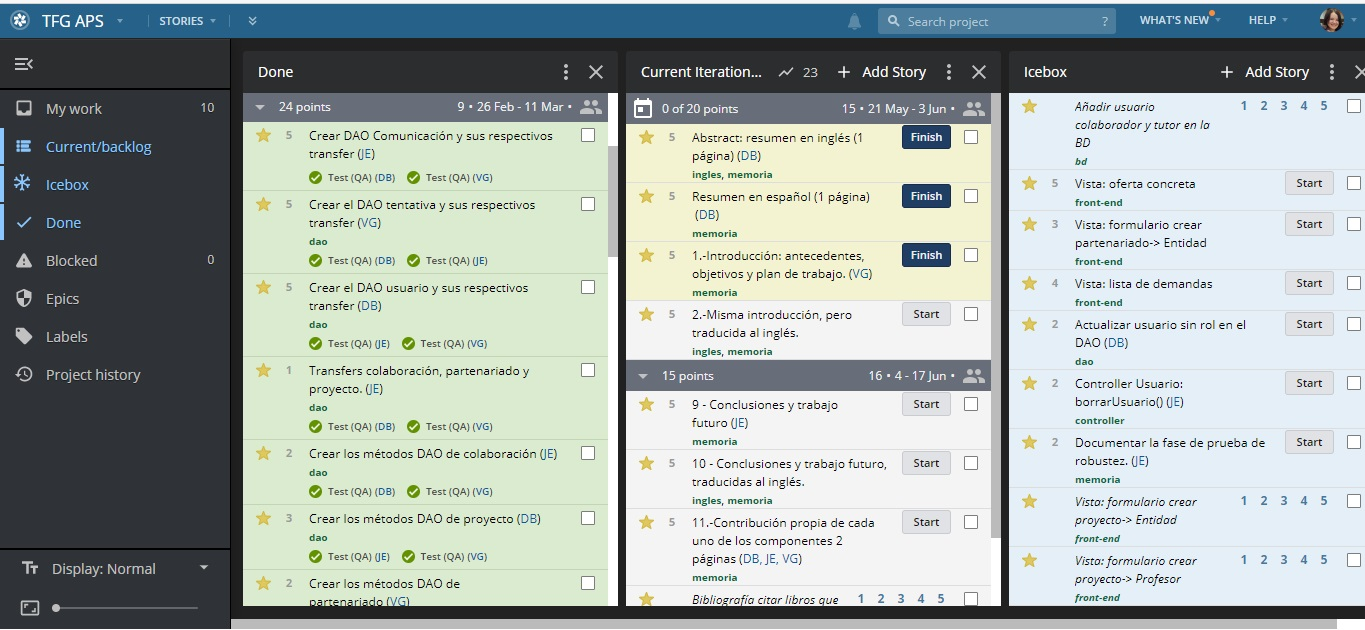
\includegraphics[scale=0.44]{pivotal2}
	\caption{PivotalTracker: tareas}
	\label{fig:pivotal2}
\end{figure}
\chapter{Contexto de la propuesta}\label{cap:contexto}
\section{Introducción}
El ApS es una propuesta educativa que combina aprendizaje y servicios a la comunidad. Los proyectos  ApS permiten a los alumnos aprender de una forma más práctica, aplicando sus conocimientos adquiridos en clase mediante la realización de tareas útiles para la comunidad. \\\\
Además de dar a los estudiantes la oportunidad de aplicar sus conocimientos en un entorno real, el ApS les impulsa a comprender el funcionamiento de la sociedad y las responsabilidades sociales que estos tienen por formar parte de una sociedad.\\\\
Todo proyecto ApS empieza por una iniciativa relacionada con una necesidad social real que implica la ejecución de un servicio para solventarla y tiene como objetivo el aprendizaje y la reflexión del alumno.
\section{Elementos que intervienen en un proyecto ApS}
En un proyecto ApS intervienen los siguientes elementos:
\begin{itemize} 
	\item El \emph{alumno} es el individuo que aplica sus conocimientos teóricos en un entorno físico beneficiando a su comunidad. Además de adquirir habilidades prácticas relacionadas con su formación, es importante que se incite al alumno a reflexionar sobre sus actos y el impacto positivo que tienen estos sobre los demás. Esto permite al alumno adquirir compromiso social y desarrollar pensamiento ético, cultivando un ciudadano responsable capaz de mejorar la sociedad de la que forma parte.
	
	\item El \emph{socio comunitario} es una empresa pública o de tercer sector que colabora con la institución educativa para resolver un determinado problema social. El socio comunitario suele tener en mente un problema muy concreto, pero no lo suficientemente detallado para la creación de un proyecto educativo. Es por eso que es necesario el partenariado. Es importante que la universidad haga entender al socio comunitario que el ApS no es voluntariado. Por tanto, bajo ningún concepto se puede usar al alumno para la generación de beneficios propios de la empresa o la competencia desleal. El principal objetivo del ApS es formar al alumno introduciéndolo en un entorno real para que este establezca una relación entre lo aprendido en el aula con lo realizado en el proyecto ApS.
	
	\item El \emph{profesor} es el individuo que se encarga de guiar al alumno en todo el proceso del proyecto, evaluando sus tareas e incitando al alumno a la reflexión. Además de guiar al alumno en su formación y gestionar el proyecto, ofrece su formación y conocimientos al socio comunitario con la que se colaborará en el proyecto. El profesor se encarga de acordar y organizar los proyectos con el socio comunitario, estableciendo todos los requisitos necesarios para la correcta formación del alumno y el cumplimiento de el socio comunitario con los principios del ApS.
	
	\item El \emph{partenariado} es una colaboración entre un profesor, o un equipo de profesores, y el socio comunitario. Partiendo de un problema social real y los conocimientos dispuestos por el profesor, el profesor y el socio comunitario determinan las características y particularidades del problema. Una vez definidos los términos y condiciones del futuro proyecto, el profesor abre el proyecto a otros profesores que quieran colaborar en la propuestas y posteriormente el proyecto se abre a los alumnos.
	\item El \emph{proyecto} consiste en la ejecución de ciertas tareas realizadas por el alumno que están relacionadas con su formación. Estas tareas permiten al alumno establecer una relación entre lo aprendido en clase y el mundo real. Gracias a estas tareas o servicios, el alumno beneficia a su comunidad, otorgándole una satisfacción personal. El alumno es evaluado de forma continua por el equipo docente.
\end{itemize}
\section{Motivación}\label{cap:cont-motidvacion}
La motivación descrita a continuación ha sido extraída de nuestros directores los cuales conocen el histórico del proyecto:\\
La experiencia de los profesores que han llevado a cabo, o intentado
llevar a cabo, iniciativas de tipo ApS muestra
que muchos proyectos potenciales no llegan a realizarse por la
dificultad en casar la oferta con la demanda, es decir, cuadrar las
necesidades didácticas, organizativas, etc. de la institución educativa
que quiere prestar un servicio, con las necesidades y disponibilidad de
la organización o comunidad que quiere recibir un servicio. El
establecimiento de relaciones de partenariado en el ApS requiere tiempo
y energía, siendo el análisis de compatibilidad entre la oferta y la
demanda de servicios un aspecto clave. Los profesores con experiencia en
iniciativas de tipo ApS, tanto de carácter local como en el contexto de
proyectos de cooperación internacional para el desarrollo, se dieron
cuenta hace tiempo de que un buen soporte informático podría ser de gran
ayuda en la difícil tarea de casar la oferta y la demanda de ApS.
Gracias a este soporte se facilitarían la identificación de potenciales
partenariados, así como la colaboración entre el prestador y el receptor
potenciales del servicio en la tarea de refinar una idea inicial y
convertirla en una propuesta de proyecto realista que cumple las
necesidades de las dos partes.\\\\

Los programas de ApS, ya consolidados en el continente americano, tan
solo recientemente empiezan a cobrar fuerza en las instituciones
educativas europeas, y en particular en las españolas. Los primeros
proyectos de ApS se iniciaron en nuestro país apenas hace 15 años.  El
escaso valor académico concedido hasta ahora a la práctica del ApS fuera
del ámbito de los estudios pedagógicos, ha sido motivo de que los
intentos de desarrollar la aplicación informática descrita hayan surgido
siempre en el contexto de PFC/TFG. El desarrollo de una tal aplicación
requiere una alta dedicación y no tiene valor de investigación
tecnológica, de modo que los profesores técnicamente cualificados no
tienen disponibilidad para abordarlo.\\\\

El PFC de Ingeniería Industrial de la
\emph{Universidad Politécnica de Madrid} (UPM) \cite{ref1} fue el primer intento, según
nuestro conocimiento, de desarrollar una aplicación para el soporte de
la definición de PFC de cooperación (y del previo establecimiento de un
partenariado Universidad-ONG) y dio como resultado una aplicación basada
en el \emph{sistema de gestión de contenidos} (CMS) Plone. Sin embargo, su
naturaleza de prototipo, junto con la falta de recursos humanos para su
despliegue y administración, hizo que nunca llegara a utilizarse.
Ángeles Manjarrés, profesora de la UNED, y Simon Pickin, uno de los directores del presente
trabajo, retomaron la idea de \cite{ref1} en el TFG del grado en Informática de
la UNED \cite{ref2}, en el que se desarrolló una aplicación web basada en el
popular \emph{framework de gestión de contenidos} (CMF) Drupal. El prototipo
desarrollado fue bastante básico e incompleto y tenía restricciones
técnicas que limitaban su funcionalidad, pero constituyó un pequeño
avance hacia el objetivo. Aunque el propósito del PFC \cite{ref1} y del TFG \cite{ref2}
fue el soporte de la definición de PFC/TFG de cooperación, este objetivo
puede verse como un caso particular del soporte de proyectos ApS y la
plataforma informática necesaria es prácticamente idéntica en los dos casos.
\\\\
Se retomó la iniciativa de \cite{ref2} en el contexto de una colaboración entre
la UCM y el grupo de investigación en innovación docente COETIC (“Grupo
de Innovación Docente de la UNED para el Desarrollo de la Competencia
Ética y Cívica y las metodologías basadas en la Comunidad en la
educación superior”) con el TFG del grado en Educación Social de la UNED
\cite{ref3}, centrado en la especificación de una aplicación para el soporte del
ApS virtual, y los TFG del grado en Informática de la UNED \cite{ref4} y \cite{ref5},
centrados en el desarrollo de tal aplicación, los dos últimos
codirigidos por Ángeles Manjarrés y Simon Pickin. En \cite{ref4}, después de un
intento fallido de continuar con el desarrollo en Drupal empezado en
\cite{ref3}, debido a que Drupal resultó ser mucho más cerrado de lo esperado,
se desarrolló una nueva aplicación desde cero basada en el stack MyEAN
(\emph{MySQL-Express-Angular-Node}). Esta aplicación se describe brevemente en
\cite{ref6}. En \cite{ref5}, se continuó el desarrollo de la aplicación de \cite{ref4} pero esta
vez con el stack MEAN (\emph{MongoDB-Express-Angular-Node}); la substitución de
MySQL por MongoDB no se debía a razones técnicas sino a razones de
conveniencia y familiaridad del desarrollador. Aunque los títulos de \cite{ref4}
y \cite{ref5} hacen referencia al ApS "Virtual", la aplicación desarrollada está
pensada para dar servicio a toda la comunidad de ApS.


\section{TFG de partida}
El TFG de David Jiménez presentaba una base a partir de la cual hemos partido para desarrollar nuestra parte de este proyecto. Partiendo del TFG anterior que estaba desarrollado en Angular y Node.js, David Jiménez siguió desarrollando la aplicación hasta conseguir un prototipo de la futura aplicación.\\\\
David Jiménez implementó las páginas de registro, \textit{login}, perfil, iniciativa y partenariado. También incluyó diferentes perfiles como el \textit{admin}, el socio comunitario, el profesor y el alumno.\\\\
 Por razones de comodidad y familiarización con la tecnología, en el TFG anterior se construyó la base de datos en MongoDB. Debido a que los datos de la aplicación son claramente estructurados y muy relacionados entre si, no había razones suficientes para seguir desarrollando la aplicación sobre MongoDB, así que junto con nuestros directores decidimos cambiar la base de datos a SQL.\\\\
Debido a las dificultades provocadas por la pandemia del COVID-19, las bases de la aplicación no quedaron del todo definidas en el TFG anterior y por esta razón hemos tenido que redefinirlas creando un modelo de dominio y de datos que representa todos los elementos del problema y cómo se relacionan entre si. Diseñamos una base de datos nueva más compleja y rica en detalles que servirá como cimientos para nuestros sucesores, ya que esperamos que llegue el día en que esta plataforma sirva a usuarios reales, los cuales ayudaran a que la educación sea más eficaz y enriquecedora.
 
\section{Estudio tecnológico}
 A continuación, se explicará qué tecnologías tienen el potencial para desarrollar este proyecto y cuáles hemos elegido finalmente. Las razones de las decisiones tomadas sobre el uso de estas tecnologías se detallan en la sección 4.
\begin{enumerate} 
	\item Servidor web:
	\begin{itemize} 
		\item ExpressJS es un \textit{framework} basado en NodeJS que permite gestionar el servidor de una forma sencilla. Este \textit{framework} fue utilizado por David Jiménez en el TFG precursor y se ha mantenido.
	\end{itemize}
	\item \emph{Backend}: 
	\begin{itemize} 
		\item NodeJS es entorno basado en JavaScript muy popular. Este entorno fue usado en el anterior TFG y se ha mantenido.
	\end{itemize}
	\item \emph{Frontend}
	\begin{itemize} 
		\item Angular es un \textit{framework} utilizado en el \textit{frontend} del TFG anterior y se ha decidido mantener.
	\end{itemize}
	\item Base de datos: 
	\begin{itemize} 
		\item MongoDB es un sistema de base de datos no estructurado. Este sistema es el que se estaba usando en el proyecto.
		\item MySQL: es un sistema de base de datos relacional. Decidimos utilizar este sistema en nuestro TFG.
	\end{itemize}
	\item Software de control de versiones:
	\begin{itemize} 
		\item Git es el controlador de versiones más conocido y muy eficaz, así que desde el principio supimos que es el software que íbamos a usar. 
	\end{itemize}
	\item Repositorio: 
	\begin{itemize} 
		\item GitHub es un repositorio gratuito que permite almacenar todos los archivos relacionados con un proyecto y mantenerlos de forma colaborativa con otros usuarios. Se ha decidido utilizar GitHub por su integración con Git.
		\item Google Drive: es un contenedor gratuito que permite almacenar cualquier fichero y compartirlo con los demás. En un principio se estudió utilizar para guardar los \textit{Backups} pero se acabó descartando. Al final se ha utilizado para almacenar todo tipo de documentos relacionados con el TFG, excepto el código fuente de la aplicación.
	\end{itemize}
	\item Herramientas de organización: 
	\begin{itemize} 
		\item GitHub Projects es una herramienta que ofrece GitHub que permite crear una organización de proyecto tipo Kanban.
		\item Trello es una herramienta sencilla estilo Kanban para organizar los proyectos, pero tiene muchas limitaciones en su versión gratuita.
		\item PivotalTracker es una herramienta de gestión de proyectos basada en Scrum que permite crear \textit{Stories}, asignarles un peso en función de lo compleja que sea la \textit{Story} y ofrece analíticas que permiten analizar el progreso del proyecto. Hemos decidido utilizar esta herramienta para organizarnos porque es una herramienta completa.
	\end{itemize}
	\item Herramientas UML: 
	\begin{itemize} 
		\item Diagrams.net es una herramienta de diseño de diagramas \textit{online} la cual permite diseñar varios tipos de diagramas entre los cuales se encuentran diagramas de clases, de flujos, de entidades, etc.
		\item Modelio es una aplicación de escritorio que permite crear modelos UML complejos, indicando los atributos, los métodos y las relaciones que tienen los elementos entre sí. Debido a que es una herramienta completa y que es una herramienta que ya conociamos, la hemos elegido para la creación de nuestros modelos.
	\end{itemize}
	\item Herramientas para el diseño del modelo relacional de la base de datos: 
	\begin{itemize} 
		\item phpMyAdmin es una herramienta web que permite gestionar una base de datos SQL. Esta herramienta muestra un modelo relacional de la base de datos muy simple.
		\item MySQL Workbench es una herramienta de gestión de diseño de base de datos visual que permite crear modelos relacionales complejos. Esta es la aplicación que se ha decidido utilizar.
	\end{itemize}
	\item Herramientas para la redacción de la memoria:
	\begin{itemize} 
		\item Microsoft Word siendo una herramienta popular y muy conocida para la creación de documentos escritos, fue nuestra primera opción para la redacción de la memoria.
		\item LaTeX es una herramienta que permite crear documentos profesionales con resultados profesionales. Esta es la herramienta que se ha decidido utilizar.
	\end{itemize}
	\item Lenguaje para insertar datos en la BD:
	\begin{itemize} 
		\item Python se ha utilizado para insertar valores enumerados en la base de datos.
	\end{itemize}
\end{enumerate}

\chapter{Modelos de dominio, de datos y de relación}\label{cap:modelos}

\section{Introducción}
Al empezar con el proyecto, junto con nuestros directores, nos hemos dado cuenta de que la aplicación necesitaba ser definida de una forma más detallada. En TFGs anteriores se entendía que los profesores y las entidades definían los proyectos de la misma forma, pero esto no es así. Las entidades no conocen todos los detalles del problema en cuestión que quieren resolver, dentro del marco de los proyectos ApS. Los profesores, por su parte, tienen una idea muy vaga del problema que quieren resolver. Normalmente tienen ciertos conocimientos académicos los cuales quieren aplicar para mejorar el mundo, pero la necesidad social en cuestión no suele estar muy clara.\\\\
En el TFG precedente se creó un elemento llamado \emph{Iniciativa} que almacenaba algunas de las características generales que comparten las propuestas del profesor y el socio comunitario. La \emph{Iniciativa} derivaba en un formulario que se les ofrecía a las entidades y a los profesores, pero las entidades y los profesores no plantean los problemas de la misma manera. Las entidades tienen una idea de proyecto clara pero no saben como orientarlo al mundo académico y los profesores tienen una idea de proyecto abstracta y lo plantean con el objetivo de encajar en un plan académico, es por esto que no es apropiado utilizar el mismo formulario para ambos.\\\\
Para definir con precisión el funcionamiento correcto y completo de la aplicación, se ha creado un modelo de dominio y un modelo de datos.
Estos modelos nos permitirán entender acertadamente el funcionamiento de la aplicación, pero lo que es más importante, permitirán transmitir dicho funcionamiento e idea general a otras personas que trabajarán en este proyecto después de nosotros.\\\\
Gracias al modelo de dominio podemos entender qué elementos intervienen y cómo interactúan entre sí, además de las restricciones que se presentan en sus interacciones.\\\\
Con el modelo de datos podemos conocer información detallada de cada elemento que interviene en la resolución del problema así como los atributos que posee.\\\\
Como se ha rediseñado la base de datos se ha decidido crear un modelo relacional que muestra todas las tablas de la nueva base de datos y sus relaciones. De esta manera, podemos representar sus especificaciones técnicas para comprender su estructura y funcionamiento. 

\section{Modelo de dominio}
El modelo de dominio es un mapa conceptual de la aplicación que permite a cualquier individuo entender su funcionamiento. El modelo de dominio de esta aplicación se puede observar en la Figura ~\ref{fig:dominio}.\\\\
Si empezamos mirando nuestro modelo desde arriba podemos observar que hay una clase madre, llamada Usuario y de ella se ramifican otras cinco clases que representan los cinco grupos de usuarios que tiene la aplicación.\\
\begin{itemize} 
	\item Los estudiantes se dividen en internos y externos. Los internos representan a aquellos estudiantes que pertenecen a la universidad donde está instalada la aplicación y los externos pertenecen a otras universidades.
	\item El grupo de usuarios promotor se divide en externos e internos por el mismo motivo que los estudiantes. 
	En promotor externo representaríamos al profesor externo, que es aquel profesor que no forma parte de la universidad donde está la aplicación pero, puede participar en un proyecto o partenariado evaluando y guiando a un estudiante externo. El colaborador, por otra parte, es un experto en algún tema en concreto que puede participar en un proyecto o partenariado ofreciendo sus conocimientos o habilidades.
	\item El promotor interno puede ser un profesor o un tutor de la universidad donde se aloja la aplicación. Este profesor es el que más cargos de responsabilidad tiene. Él es el que puede crear las ofertas de servicio y es el responsable de crear los partenariados y los proyectos.
	\item El socio comunitario es aquella entidad que hace de socio para la creación del proyecto.
	\item El admin es el usuario administrador de la aplicación.
	\item La Oficina APS es un usuario responsable de todos los tramites relacionados con la gestión de los proyectos ApS. 
\end{itemize}
Todo proyecto tiene que definirse en el contexto de un partenariado y este partenariado se origina en la unión de una oferta creada por un profesor, y una demanda creada por un socio comunitario. La creación de la oferta y la demanda se realiza mediante unos formularios en la web.\\
La aplicación también contempla la
creación de partenariados ``monoparentales'', es decir, partenariados
creados cuando un socio comunitario acepta una oferta creada por un
profesor sin haber creado previamente una demanda, o cuando un profesor
respalda una demanda creada por un socio comunitario sin haber creado
previamente una oferta. En estos casos, la correspondiente oferta (resp.
demanda) se creará en el momento de aceptar (resp. respaldar) la oferta
(resp. la demanda) y se utilizará un atributo de la oferta y de la
demanda para almacenar la naturaleza ``monoparental'' del partenariado.\\
En general una demanda de servicio es creada por una socio comunitario, pero puede llegar a crearse gracias a un estudiante, el cual previamente ha tenido que crear una iniciativa. Una iniciativa es una propuesta de proyecto de un estudiante, la cual es acogida posteriormente por un socio comunitario. Cuando el socio comunitario acoge dicha iniciativa, esta se convierte en una demanda de servicio.\\
Debido a que los proyectos definidos por los profesores y los definidos por las entidades comparten ciertas características, podemos ver en el diagrama que ambos cuelgan de un elemento padre llamado Anuncio de servicio que posee las características comunes de ambos.
Lo mismo ocurre con partenariado y proyecto que cuelgan de Colaboración Uni-Ent.\\
Queremos destacar que los atributos de Necesidad social y Area de implementación, tan importantes para emparejar ofertas y demandas, han sido obtenidos de la página web \url{www.eoslhe.eu/resources/}
Los partenariados y los proyectos presentan ciertas restricciones relacionadas con la participación de alumnos y promotores externos.\\\\
En los proyectos solo pueden participar estudiantes externos si el responsable del proyecto acepta estudiantes externos. 
Los profesores externos solo pueden participar en aquellos partenariados y proyectos que los acepten. Además, en el caso de un proyecto, un participante solo puede tener el
perfil de profesor externo si también participan alumnos externos de su
universidad, cuya participación tendrá que evaluar; en otro caso, tendrá
el perfil de colaborador, independientemente del tipo de puesto que
ocupa en su universidad.\\\\
\begin{landscape}
	\begin{figure}[p]
		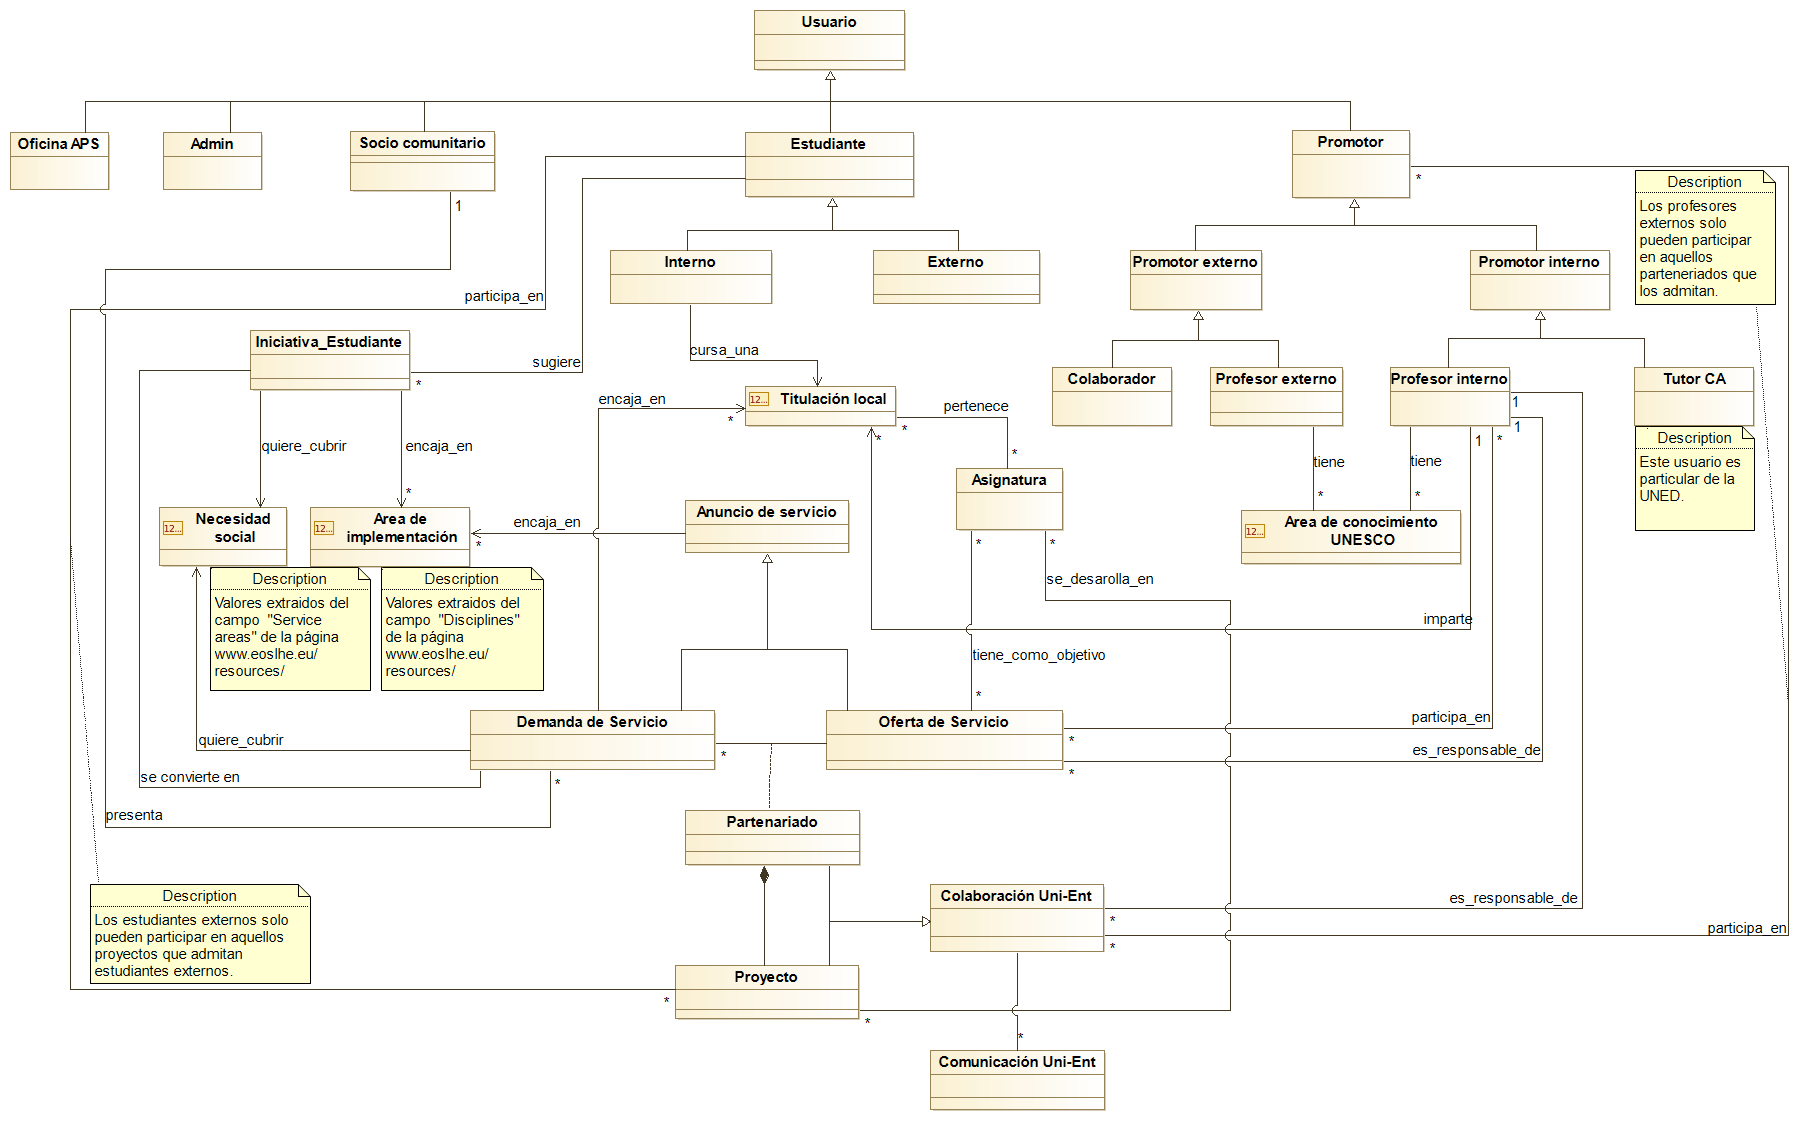
\includegraphics[scale=0.4]{mdominio}
		\caption{Modelo de dominio}
		\label{fig:dominio}
	\end{figure}
\end{landscape}
\begin{landscape}
	\begin{figure}[p]
		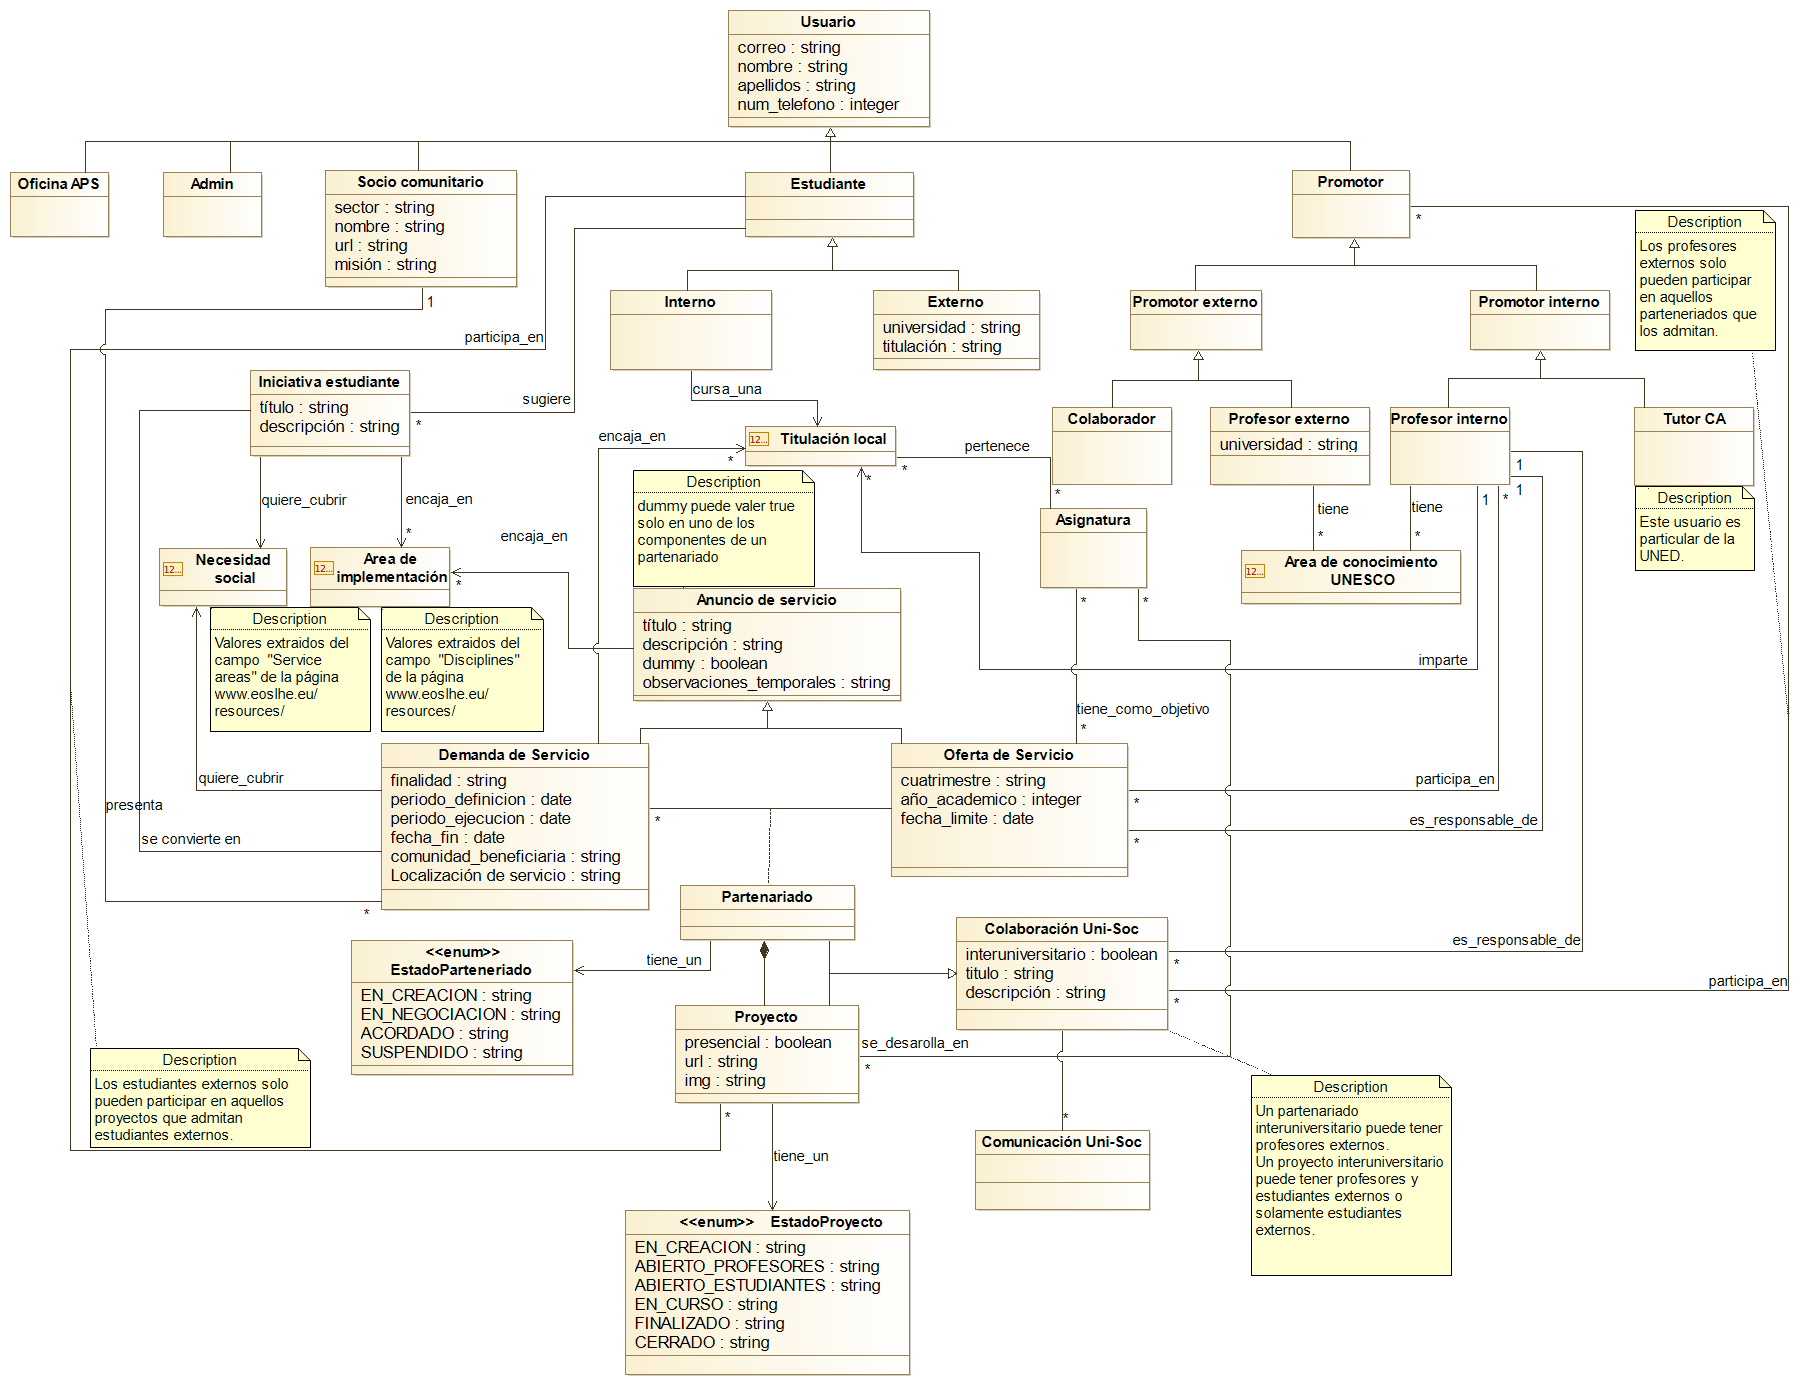
\includegraphics[scale=0.35]{mdatos}
		\caption{Modelo de datos}
		\label{fig:datos}
	\end{figure}
\end{landscape}

\section{Modelo de datos}
El modelo de datos describe con más precisión el dominio de la aplicación.
Además de algunos atributos importantes como el interuniversitario, que indica si el partenariado o el proyecto está abierto a externos, podemos observar los estados que pueden tener el partenariado y el proyecto, representados por dos enumerados. En particular podemos ver que el partenariado puede encontrarse en estados \texttt{EN\_CREACION}, \texttt{EN\_NEGOCIACION}, \texttt{ACORDADO} y \texttt{SUSPENDIDO}. El modelo de datos se puede observar en la Figura ~\ref{fig:datos}.\\
\begin{itemize} 
	\item El partenariado toma el estado de \texttt{EN\_CREACIÓN} cuando el profesor se pone en contacto con el socio comunitario o el socio comunitario se pone en contacto con el profesor. Si el receptor de la propuesta contesta y acepta colaborar con el otro, el estado del partenariado pasará a \texttt{EN\_NEGOCIACION}. Cuando el profesor y el socio comunitario terminan de establecer los términos y condiciones del partenariado y ambos están de acuerdo con dichos terminos, el partenariado pasá a estar \texttt{ACORDADO}. Si ocurre cualquier discrepancia durante la fase de \texttt{EN\_CREACION}, \texttt{EN\_NEGOCIACION} o \texttt{ACORDADO} el partenariado puede pasar al estado de \texttt{SUSPENDIDO}.\\\\
	\item El proyecto toma los estados \texttt{EN\_CREACION}, \texttt{ABIERTO\_PROFESORES}, \texttt{ABIERTO\_ESTUDIANTES}, \texttt{EN\_CURSO}, \texttt{FINALIZADO} y \texttt{CERRADO}.
	El profesor interno responsable de un partenariado en estado \texttt{ACORDADO}  puede pedir que se cree un proyecto derivado de este partenariado. El
	estado inicial de un proyecto es \texttt{EN\_CREACIÓN}. Cuando el socio
	comunitario da su asentimiento a la creación del proyecto, su estado
	pasa a ser \texttt{ABIERTO\_PROFESORES}. Una vez terminada la definición del proyecto se abre a los alumnos y es allí cuando el proyecto pasa al estado de \texttt{ABIERTO\_ESTUDIANTES}. Si el proyecto finaliza correctamente, pasará al estado de \texttt{FINALIZADO}. Si sucede cualquier imprevisto durante las 4 fases anteriores el proyecto puede pasar al estado \texttt{CERRADO}.
\end{itemize} 

\section{Modelo relacional}
 Debido a la complejidad de la nueva base de datos compuesta por 46 tablas relacionales, se ha decidido crear un diagrama que sirva como mapa en la gestión de la base de datos. Este modelo relacional se divide en cuatro secciones claramente diferenciadas.
 \begin{itemize} 
 	\item La sección de los usuarios que contiene tablas relacionadas con información de los usuarios. La sección del Anuncio de servicio que contiene todas las tablas que representan información de las ofertas de servicio, las demandas de servicio y las iniciativas.
	\item La sección de Colaboración contiene la información relacionada con los partenariados y los proyectos.
	\item La sección de Comunicación que contiene las tablas de \textit{mail}, mensaje, \textit{upload} y \textit{newsletter}, estas fueron creadas por David Jiménez en los documentos de MongoDB cuya estructura se ha mantenido intacta.
	En la Figura \ref{fig:relacional} se puede observar el modelo relacional y sus cuatro secciones separadas por colores.
\end{itemize}
\begin{landscape}
	\begin{figure}[p]
		\centering
		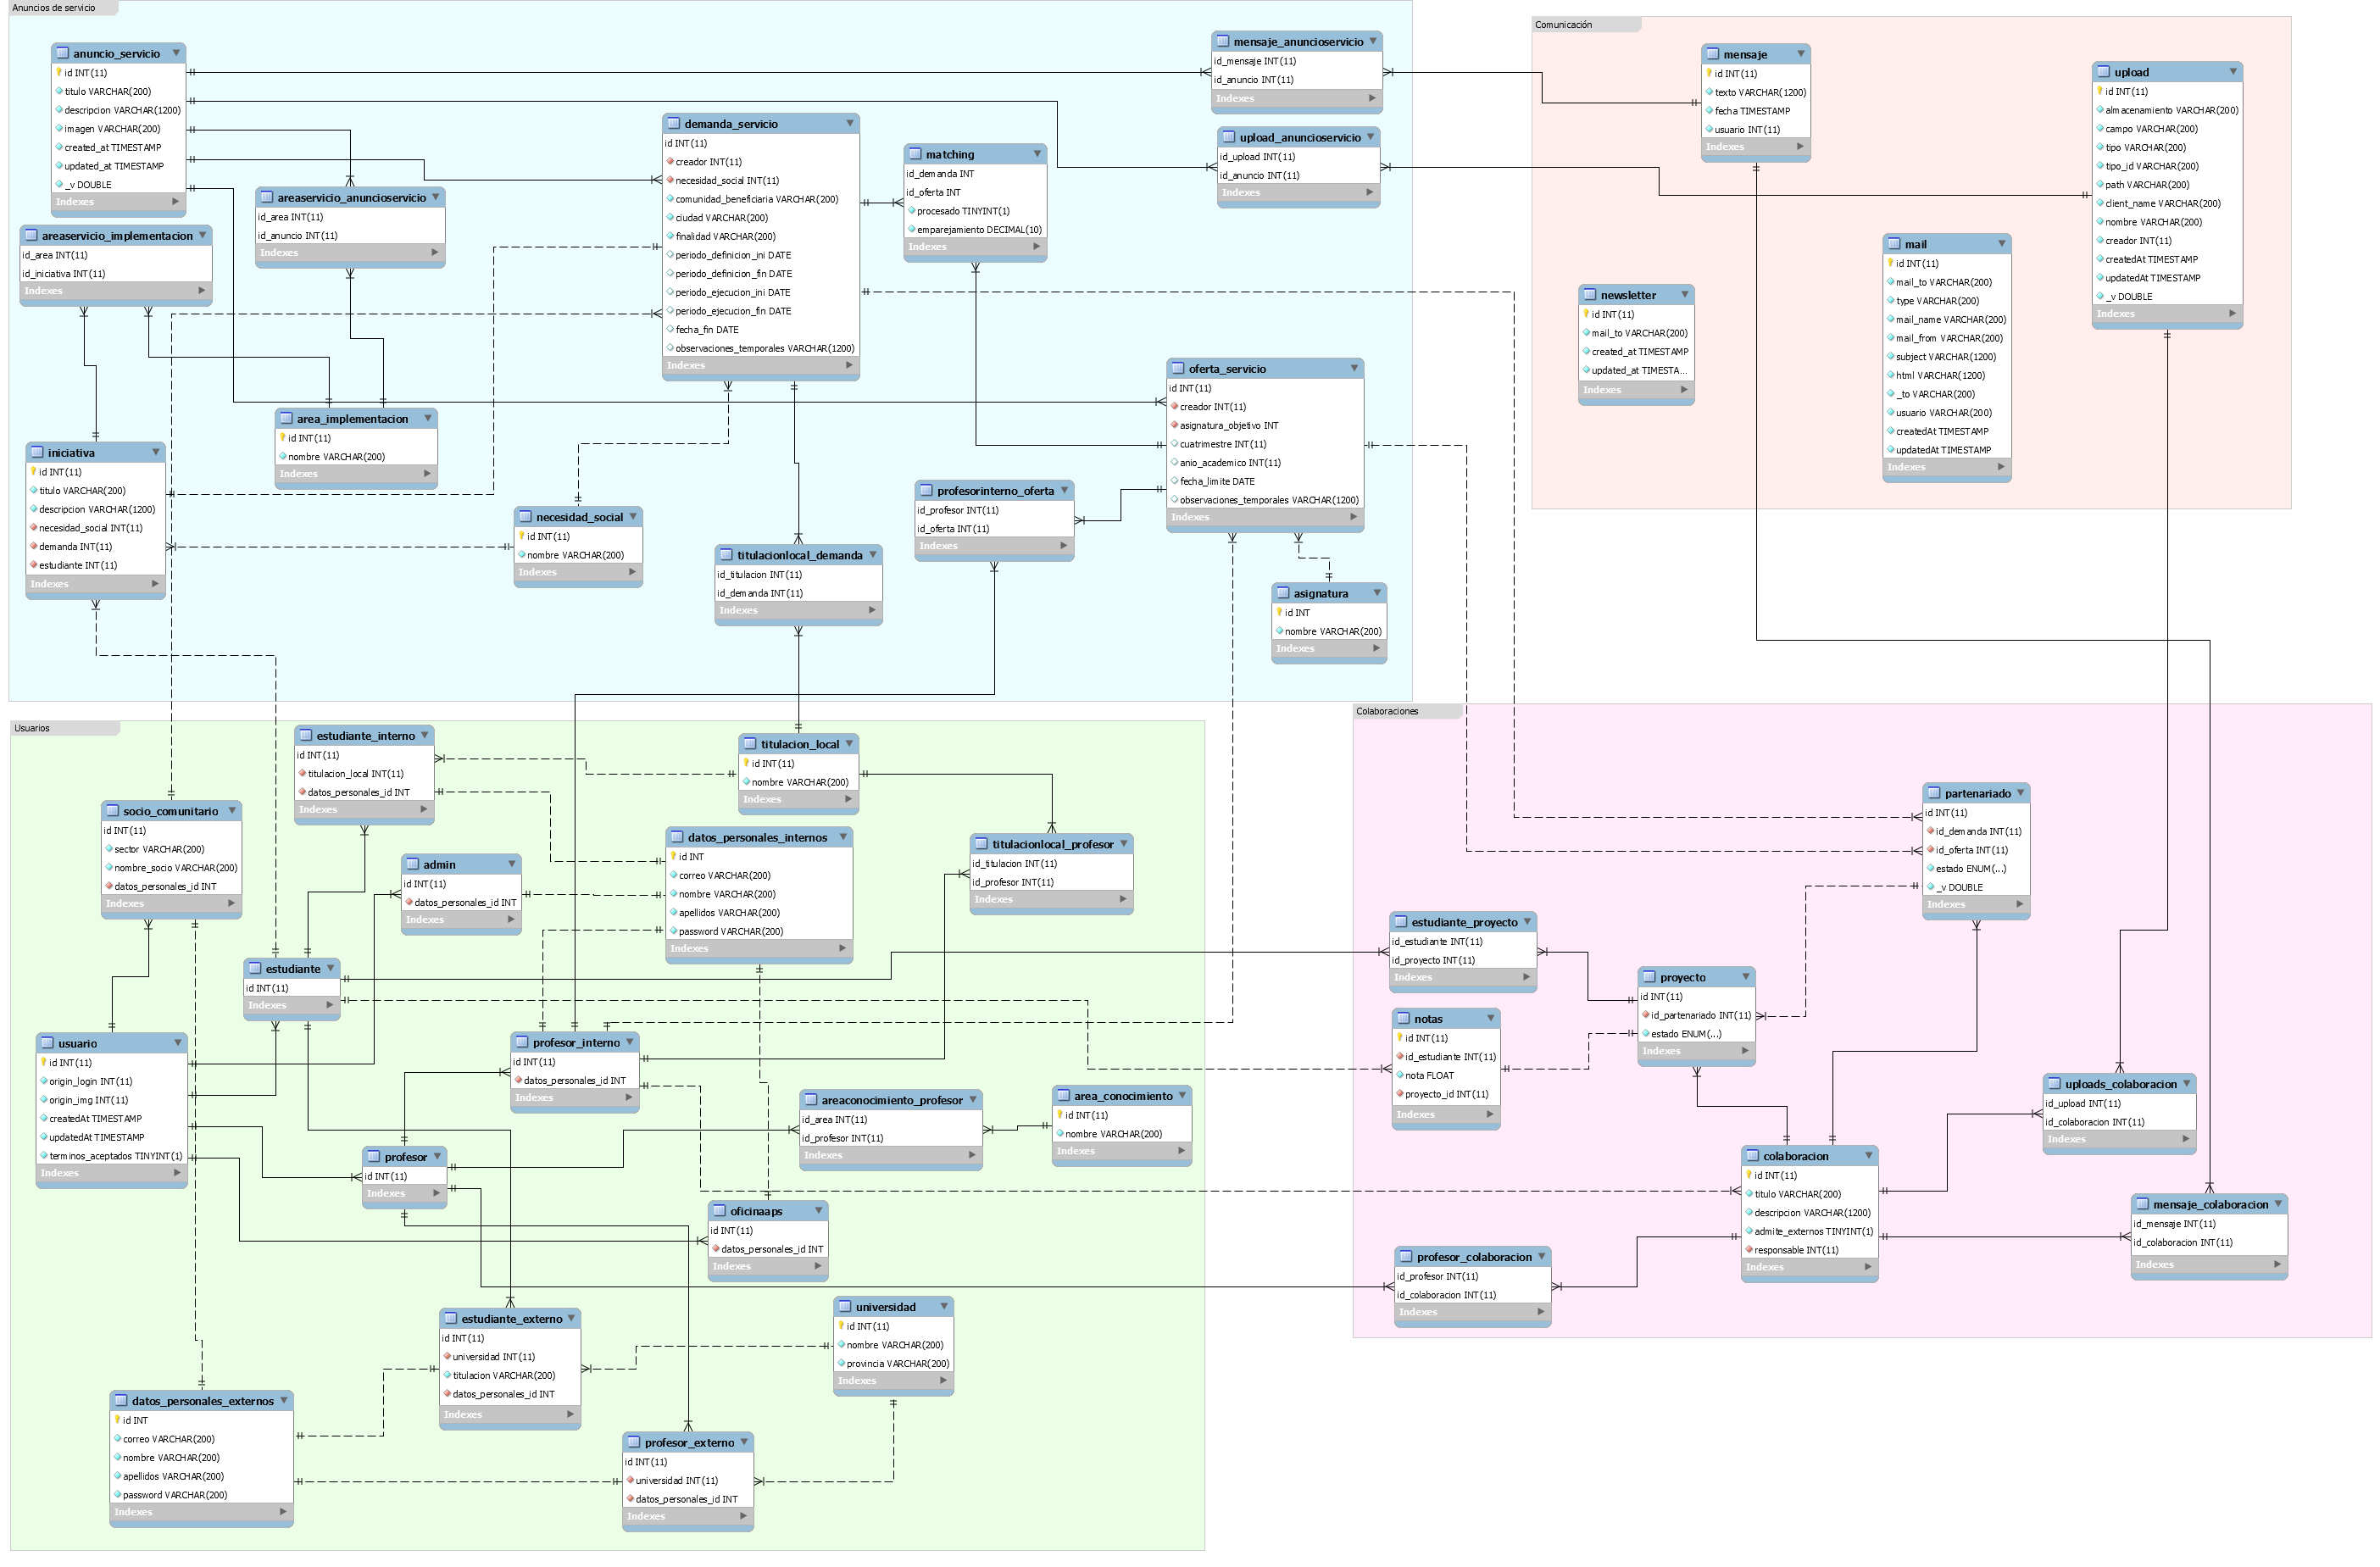
\includegraphics[scale=0.27]{er}
		\caption{Diagrama de entidad-relación}
		\label{fig:relacional}
	\end{figure}
\end{landscape}

\subsection{Separación de datos}
Una cosa importante a destacar es que, en un entorno real, la aplicación cogería parte de los datos de los usuarios de la base de datos de la universidad en la que se despliegue la aplicación. Es por esto que los datos de los usuarios se han separado en dos grupos; internos y externos. Los usuarios internos son aquellos que pertenecen a la universidad en la que se ha desplegado la aplicación y por ello utilizan SSO (Single Sign-On) para acceder a la aplicación. Esta separación de datos se ha hecho con el propósito de facilitar la transición entre la base de datos del prototipo y la base de datos de la aplicación real.\\
En concreto, los datos que son afectados por esta separación son el correo electrónico, el nombre, los apellidos y la contraseña que deberían alojarse en la base de datos de la universidad.
\subsection{Usuarios}
Esta sección es la más compleja debido a la separación que hay que realizar de los usuarios externos e internos. Ver Figura \ref{fig:usuarios}.\\
Un usuario interno es aquel profesor, tutor, estudiante, administrador o representante de la oficina ApS que forma parte de la universidad en la que se despliega la plataforma y por tanto tiene sus datos personales dentro de ella. Debido a que en un despliegue real, tendrían parte de los datos que necesitamos para la aplicación en el sistema interno de la universidad, hay que tratarlos de manera diferente a los usuarios externos, que son aquellos que no pertenecen a la universidad. Los colaboradores y directores que aquí mencionamos se pueden ver representados en el modelo de datos y de dominio, pero no se observan aquí porque no nos dio tiempo a integrarlos en la base de datos.\\\\
Debido a esta separación, todos los usuarios comparten una tabla común, llamada usuario, que contiene datos exclusivos de la cuenta de la plataforma. Después tenemos tablas que contienen datos particulares de cada tipo de usuario. Estas son las tablas del \textit{socio comunitario}, estudiante interno, estudiante externo, \textit{admin}, profesor interno, profesor externo y oficina ApS.\\
Cada uno de estos usuarios poseen una tabla que almacena sus datos personales, haciendo diferenciación entre internos y externos. La tabla de datos\_personales\_internos es una tabla creada para la simulación de la aplicación. Una vez la aplicación sea desplegada en un entorno real, esta tabla será eliminada y los datos personales se obtendrán haciendo consultas a la base de datos de la universidad.\\
Por otra parte podemos observar tablas secundarias que representan características de los usuarios como por ejemplo, la universidad del profesor y estudiante interno, las áreas de conocimiento UNESCO de los profesores y las titulaciones que imparten los profesores o cursan los alumnos.
\begin{landscape}
	\begin{figure}[p]
		\centering
		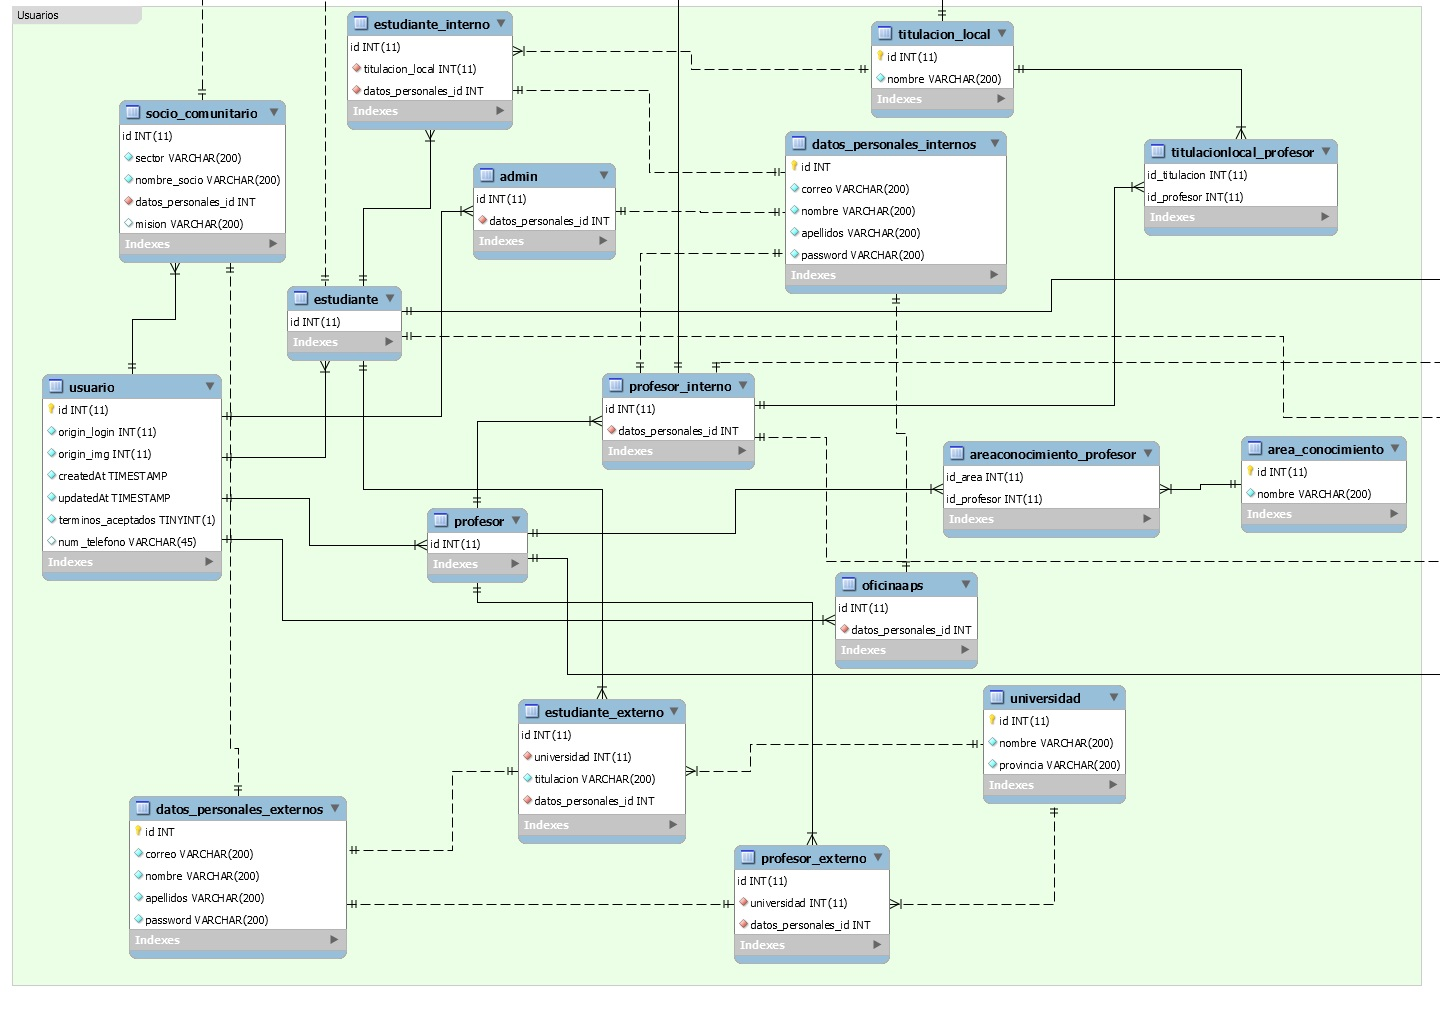
\includegraphics[scale=0.6]{usuarios}
		\caption{Diagrama de entidad-relación - Usuarios}
		\label{fig:usuarios}
	\end{figure}
\end{landscape}

\subsection{Anuncios de servicio}
En este conjunto de tablas podemos encontrar las pertenecientes a la demanda de servicio, la oferta de servicio y la iniciativa. Ver Figura \ref{fig:anuncios}.
\begin{itemize} 
	\item La iniciativa es una propuesta de proyecto realizada por un estudiante. Esta propuesta debe ser validada por la oficina ApS, que estudiará si la propuesta es viable para ser adoptada por un socio comunitario. Una vez validada la iniciativa, puede ser adoptada por un socio comunitario que desee realizar el proyecto.
	\item La demanda de servicio es creada por un socio comunitario y define una necesidad especifica que quiere cubrir. Esta necesidad social es representada por los elementos de un enumerado alojado en la tabla de necesidad\_social.
	\item La oferta de servicio es creada por un profesor interno y suele tener menos detalles que la demanda porque suele ser una propuesta más genérica.\\
	Cuando una oferta y una demanda son procesadas por el sistema de \textit{matching} se crea una entrada en la tabla \textit{matching} almacenando los \textit{ids} de ambos elementos y el porcentaje de emparejamiento que tienen.\\
	Tanto demanda de servicio como oferta de servicio están conectadas a mensajes y \textit{uploads} porque estos permiten la comunicación con las personas interesadas en las propuestas.
\end{itemize}
\begin{landscape}
	\begin{figure}[p]
		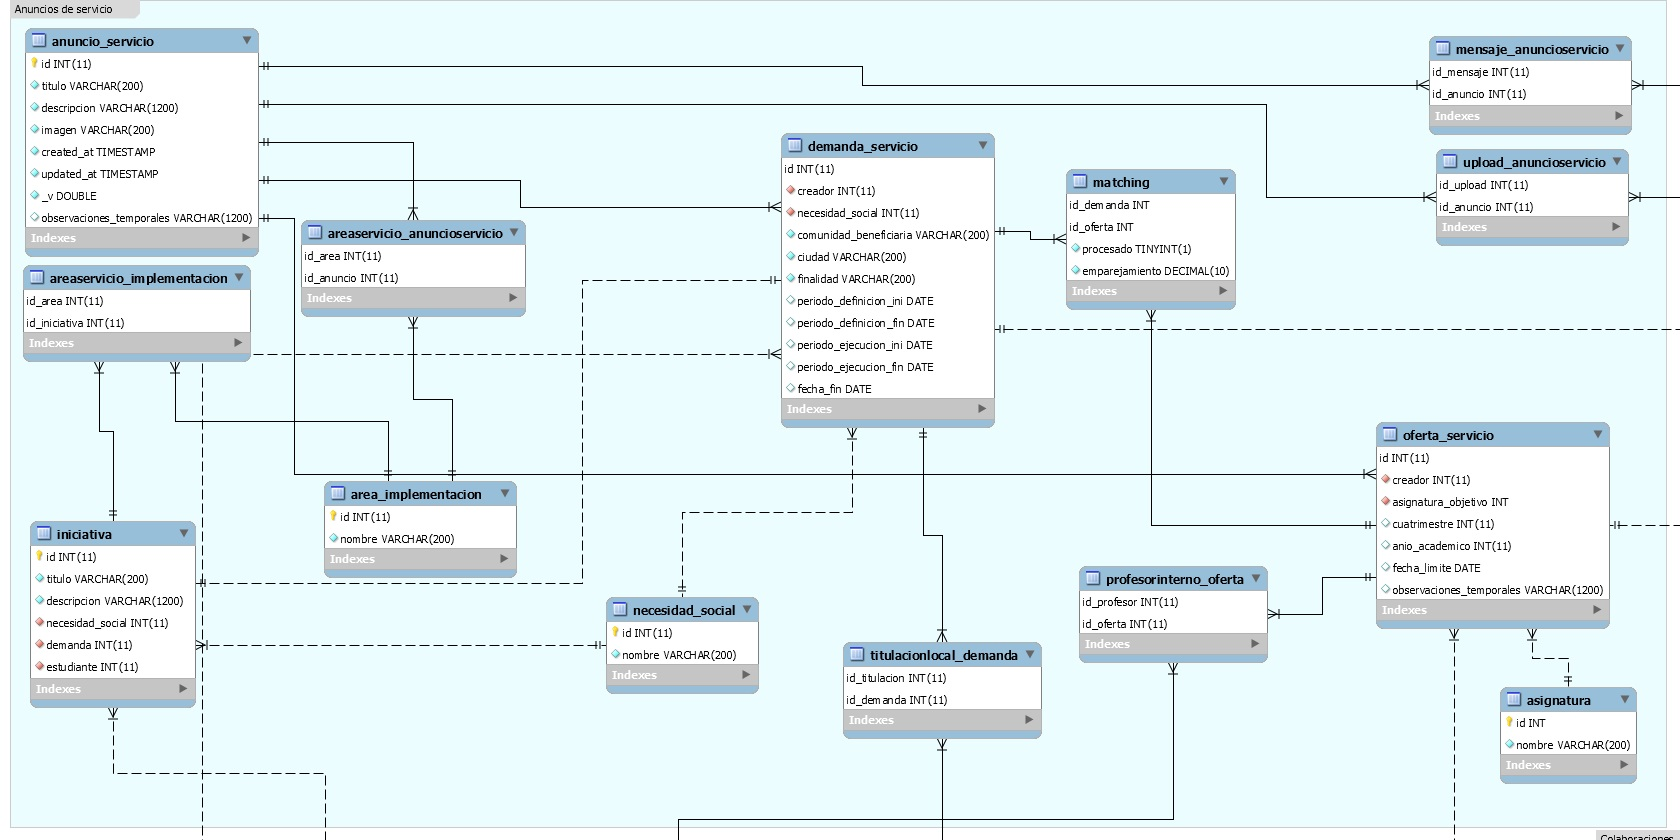
\includegraphics[scale=0.6]{anuncios}
		\caption{Diagrama de entidad-relación - Anuncios de servicio}
		\label{fig:anuncios}
	\end{figure}
\end{landscape}

\subsection{Colaboración}
El partenariado es el segundo paso en la creación de un proyecto. Esta tabla contiene los \textit{ids} de la demanda y la oferta que la componen.\\
Un proyecto ApS no puede existir sin un partenariado previo y es por eso por lo que tiene un identificador del partenariado a partir del cual se creó. El proyecto posee estudiantes y por ello tiene una conexión con los mismos.\\
Tanto proyecto como partenariado necesitan un sistema de comunicación y es por eso por lo que tienen tablas intermedias que los conectan a mensaje y \textit{uploads}. Ver Figura \ref{fig:colaboracion}.
\begin{landscape}
	\begin{figure}[p]
		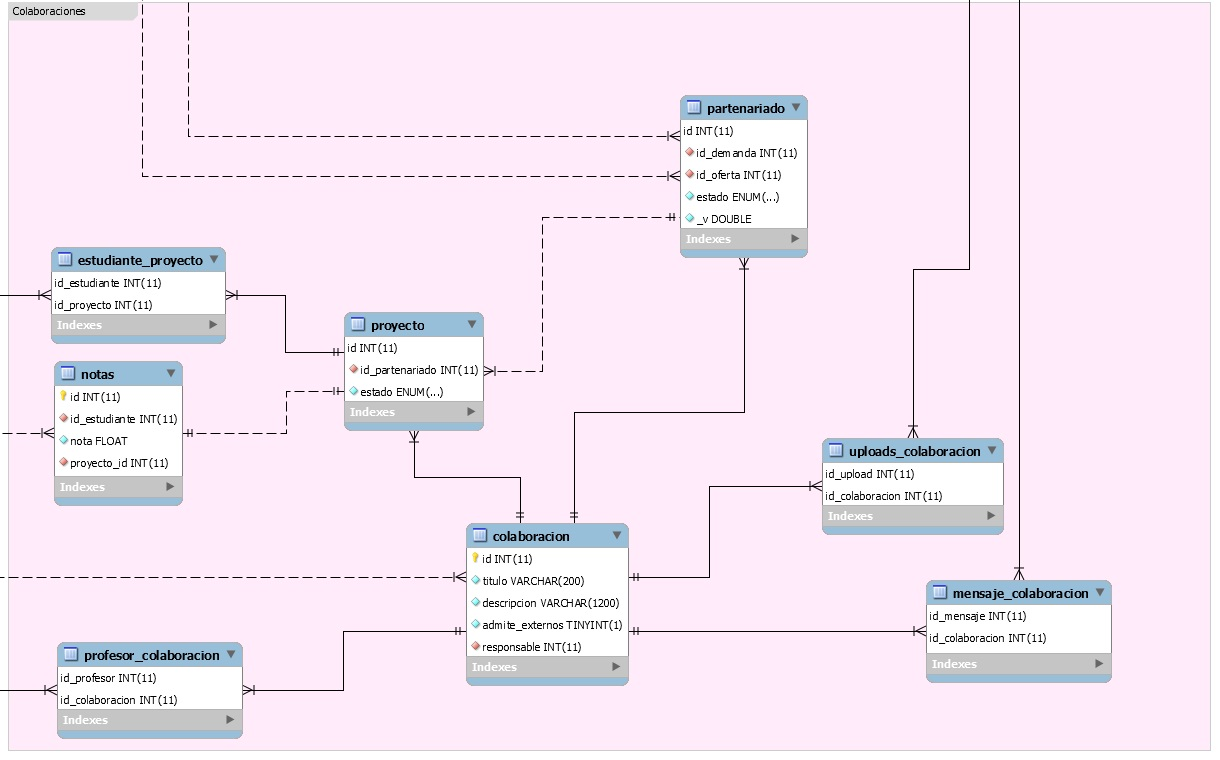
\includegraphics[scale=0.6]{colaboracion}
		\caption{Diagrama de entidad-relación - Colaboración}
		\label{fig:colaboracion}
	\end{figure}
\end{landscape}
\subsection{Comunicación}
Las funcionalidades de estas tablas no han sido del todo definidas, ya que en un principio se pensó que podrían comunicar al equipo docente con los socios comunitarios en los partenariados y los proyectos, pero también se podrían usar para la comunicación con los creadores de las ofertas y las demandas. Debido a que el funcionamiento no ha sido estudiado aun y que no hemos trabajado con estas tablas en nuestro TFG, se ha mantenido la misma estructura que había definido David Jiménez en sus colecciones de MongoDB adaptándola al modelo relacional. Ver Figura \ref{fig:comunicacion}. 
\begin{itemize} 
	\item La tabla de mensajes conecta con las ofertas de servicio, las demandas de servicio, los partenariados y los proyectos porque todos estos necesitan de los mensajes para poder comunicarse.
	\item La tabla \textit{upload} almacena la información de los ficheros e imágenes subidos tanto en ofertas de servicio, como demandas de servicio, como partenariados y proyectos.
	\item La tabla \textit{mail} y \textit{newsletter} no han sido conectadas con ninguna otra tabla porque no se han tenido en cuenta para el desarrollo de este TFG, pero representan los correos electrónicos internos de la aplicación y las noticias periódicas enviadas a los usuarios.
\end{itemize}
\begin{figure}[t]
	\centering
	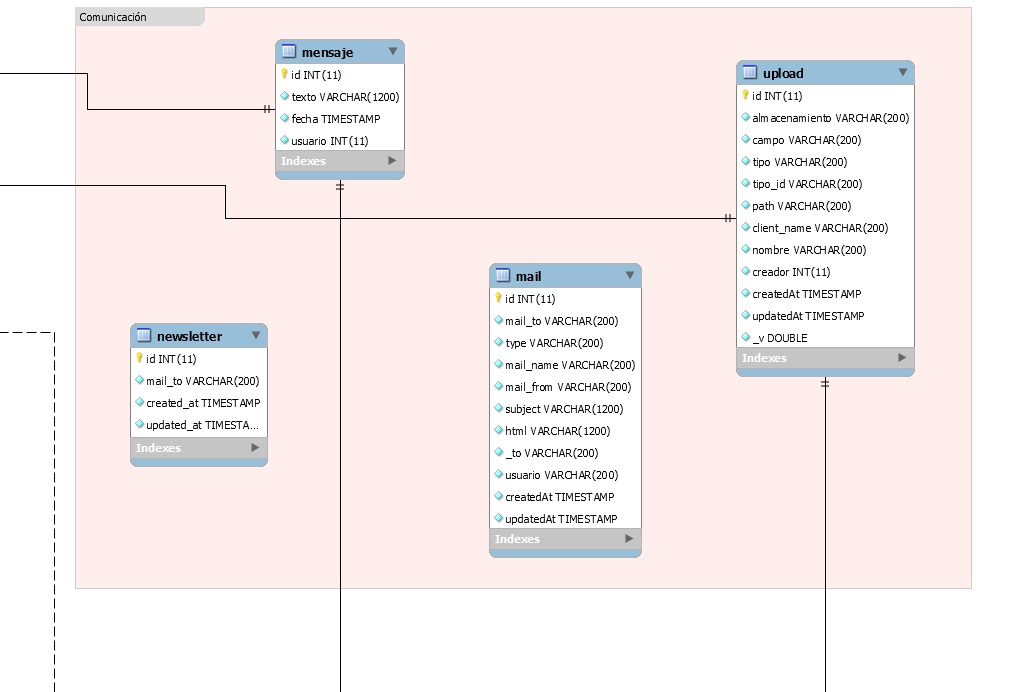
\includegraphics[scale=0.6]{comunicacion}
	\caption{Diagrama de entidad-relación - Comunicación}
	\label{fig:comunicacion}
\end{figure}

\bibliography{referencias}
\end{document}
